\chapter{Comparaison GCM - CCM - OCB}

\section{CCM}

Le mode CCM est un mode de fonctionnement qui permet à la fois l'authentification et la confidentialité. Le mode CCM est définit que pour les algorithme de chiffrement par bloc dont la taille des bloc est de 128 bits.


Le vecteur d'initialisation (IV) doit est être choisi avec précaution car il ne doit jamais être utilisé plus d'un fois par clef. En effet le mode CCM est un dérivé du mode CTR.


Comme son nom le suggère le mode CCM combine le mode CBC-MAC et le mode CTR. C'est deux mode "primitfs" sont combiné pour authentifier les données puis les encrypter. CBC-MAC permet dans un premier temps d'obtenir un tag d'authentification du message clair. Puis le message et le tag sont encryptés en utilisant le mode CTR.


Une idée essentielle est que la même clé de cryptage peut être utilisé à la fois pour l'authentification et l'encryptage, à condition que les valeurs de comptage utilisées dans le cryptage ne rentrent pas en collision avec le vecteur d'initialisation (VI) utilisé pour l'authentification.


\begin{figure}[!h]
  \centering
  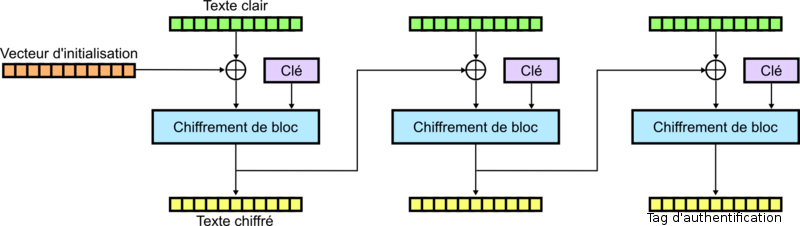
\includegraphics[width=\textwidth]{fonctionnement-CBC_MAC}
  \caption{Création du tag d'authentification avec CBC-MAC}
  \label{Création du tag d'authentification avec CBC-MAC}
\end{figure}

\begin{figure}[!h]
  \centering
  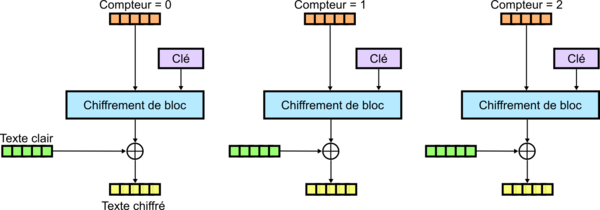
\includegraphics[width=\textwidth]{fonctionnement-CTR}
  \caption{Chiffrement du tag et du message avec CTR}
  \label{Chiffrement du tag et du message avec CTR}
\end{figure}




\section{OCB}
Le mode OCB est lui aussi conçu pour fournir à la fois l'authentification et la confidentialité. OCB (Offset CodeBook) est basé sur le mode ECB avec l'utilisation d'un vecteur d'initialisation. Pour l'authentification il faut d'abord effectuer un checksum du message clair, ce checksum est ensuite encrypter comme un block du message clair. 

\begin{figure}[!h]
  \centering
  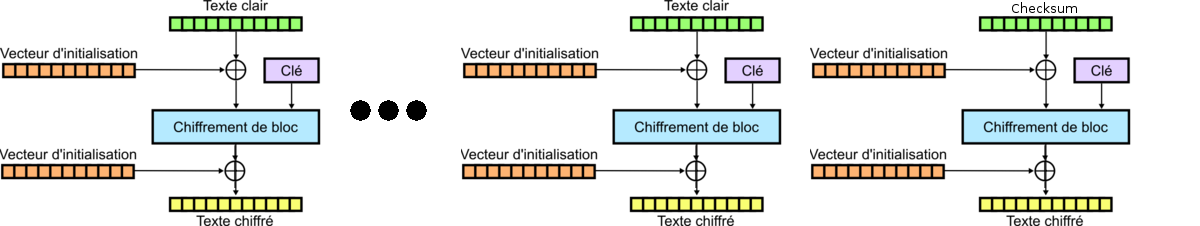
\includegraphics[width=\textwidth]{fonctionnement-OCB}
  \caption{Fonctionnement du mode OCB}
  \label{Fonctionnement du mode OCB}
\end{figure}
